\documentclass[12pt]{article}

\bibliography{sbc-template}

\usepackage{graphicx}
\usepackage{indentfirst}
\usepackage[utf8]{inputenc}
\usepackage{listings}
\usepackage{sbc-template}
\usepackage{url}

\lstset{language=[LaTeX]TeX,
        basicstyle=\ttfamily,
        columns=fullflexible,
        keepspaces=true}

\sloppy

\title{Relatório do Projeto: CPU RISC-V 32 Bits com Instruções Vetoriais}
\author{Andrés Gonzalez Vilhena\\
        David Moreira Jacinto da Silva\\
        Lucas da Silva Inocencio}

\address{Escola Politécnica da Universidade Federal do Rio de Janeiro (UFRJ)\\
  Rio de Janeiro -- RJ -- Brasil
\email{agv1@poli.ufrj.br, davidmoreirajacinto.20222@poli.ufrj.br}
\email{lucas.inocencio@poli.ufrj.br}
}

\begin{document}

\maketitle

\begin{abstract}
This project extends the original design of a 32-bit RISC-V Central Processing Unit (CPU) to support the usage of vector instructions. The enhanced CPU maintains a 5-stage pipeline and is implemented using VHDL blocks in the LogiSIM-Evolution simulator. Distinct instruction and data memories are utilized, delivering one word per cycle, and have been modified to accommodate asynchronous data loading, making use of LogiSIM-Evolution's ROM and RAM memories. The CPU is adapted to pause its operation during data loading, preserving its internal state, and includes a reset signal. For this task, the integer pipeline is exclusively implemented, specifically supporting vector versions of certain instructions.

The newly supported vector instructions include arithmetic operations (add, addi, auipc, and sub) and bitwise shift operations (sll, slli, srl, and srli). Additionally, the CPU retains compatibility with the subset of the RV32I ISA from the previous practical activity. The implementation of these new instructions adheres to the principles of the RISC-V architecture, with a detailed explanation provided in the final report.
\end{abstract}

\section{Enunciado}

Estender o projeto original da nossa CPU RISC-V de 32 Bits para suportar o uso de
instruções vetoriais. A nova CPU deve manter um pipeline com ao menos 5 estágios, e a
implementação deve ser realizada usando blocos VHDL no simulador LogiSIM-Evolution. As
memórias de instruções e dados são distintas e entregam cada uma palavra por ciclo, além
disso essas memórias devem ser modificadas para permitir carga de dados assíncrona
(pode usar as memórias ROM e RAM do LogiSIM-Evolution). A CPU deve ser adaptada
para não operar durante essa carga de dados (manter seu estado interno corrente), além de
possuir um sinal de reset. Para esta tarefa apenas o pipeline de inteiros será implementado,
especificamente as versões vetoriais das instruções a seguir devem ser suportadas:
\begin{itemize}
    \item add, addi, auipc e sub
    \item sll, slli, srl e srli
\end{itemize}
Além das instruções acima listadas, que são baseadas na atividade prática AVX,
essa CPU deve suportar o subconjunto da ISA RV32I da tarefa prática anterior. Essas
novas instruções devem ser aderentes a proposta da arquitetura RISC-V, devendo constar
no relatório final abordagem usada na codificação dessas novas instruções.


\section{Introdução}

O objetivo principal deste projeto é estender a CPU RISC-V de 32 bits desenvolvida anteriormente, que operava com instruções escalares, para incorporar suporte a instruções vetoriais. A nova CPU manterá o pipeline de 5 estágios e preservará as instruções da ISA RV32I do projeto original, permitindo compatibilidade com aplicações já desenvolvidas para essa arquitetura.

A extensão da CPU para suportar instruções vetoriais possibilitará a execução simultânea de operações em vetores de dados, aumentando significativamente o desempenho de tarefas que podem ser paralelizadas. Isso tornará a CPU mais adequada para aplicações que demandam processamento intensivo de dados, impulsionando a eficiência em áreas como processamento de sinais, aprendizado de máquina, processamento de imagens e muito mais.

O desenvolvimento do projeto foi conduzido em etapas estruturadas, permitindo uma abordagem sistemática e iterativa para garantir a qualidade e eficiência do resultado final. A metodologia de desenvolvimento incluirá:

Análise da ISA RV32I e Instruções Vetoriais: A primeira etapa consistirá em analisar detalhadamente a ISA RV32I e as instruções vetoriais que serão incorporadas à CPU. Será feita uma seleção criteriosa das instruções que serão suportadas para garantir a relevância e eficiência do projeto.

Projeto da Extensão Vetorial: Nesta fase, serão projetados os blocos funcionais necessários para adicionar o suporte a instruções vetoriais à CPU. Isso incluirá a definição dos formatos de instrução, a modificação dos estágios do pipeline e a adição de unidades funcionais específicas para o processamento de vetores.

Implementação dos Blocos VHDL: Com o projeto detalhado, a implementação dos blocos em VHDL será realizada no simulador LogiSIM-Evolution. Cada bloco será testado e validado individualmente, garantindo sua funcionalidade e integração com os demais componentes da CPU.

Modificação das Memórias e Unidade de Controle: A implementação das instruções vetoriais exigirá modificações nas memórias de instruções e dados para suportar carregamento assíncrono de dados. Além disso, a unidade de controle será adaptada para coordenar adequadamente as operações vetoriais.

Testes e Validação: Após a implementação da CPU com suporte a instruções vetoriais, serão realizados testes abrangentes e validações para garantir o correto funcionamento das instruções escalares e vetoriais em diferentes cenários de execução.


\section{Desenvolvimento}

O desenvolvimento deste projeto consistiu na extensão e aprimoramento da CPU RISC-V de 32 bits previamente desenvolvida, adicionando suporte a instruções vetoriais. A CPU original, baseada na ISA RV32I e projetada com um pipeline de 5 estágios, proporcionou uma base sólida para a implementação das instruções vetoriais, permitindo a execução simultânea de operações em múltiplos elementos de dados e aumentando significativamente o desempenho computacional em tarefas paralelizáveis.

\subsection{Análise da ISA RV32I e Seleção de Instruções Vetoriais}


A primeira etapa do desenvolvimento envolveu uma análise detalhada da ISA RV32I e das instruções vetoriais disponíveis. A seleção cuidadosa das instruções a serem incorporadas foi realizada com base na relevância e impacto no desempenho geral da CPU. Optou-se por incluir as seguintes instruções vetoriais, que complementariam o conjunto já suportado de instruções escalares:

Instruções Aritméticas Vetoriais: Foram adicionadas as operações vetoriais de adição e subtração, permitindo o processamento simultâneo de múltiplos pares de operandos. Essas instruções foram fundamentais para acelerar cálculos em aplicações como processamento de sinais e matrizes.

Instruções de Deslocamento Vetorial: As operações vetoriais de deslocamento à esquerda e à direita foram incluídas, proporcionando maior eficiência na manipulação de vetores de dados e otimizando tarefas como processamento de imagens e criptografia.

\subsection{Projeto da Extensão Vetorial}


Com a seleção das instruções vetoriais definida, o próximo passo foi projetar a extensão vetorial na CPU. Foram criados novos blocos funcionais para a execução das operações vetoriais e adaptados os estágios do pipeline para suportar o processamento de vetores. As unidades funcionais, como a Unidade Lógica e Aritmética (ALU), foram expandidas para operar com vetores de dados, tornando a CPU capaz de realizar cálculos em paralelo.


\subsection{Implementação dos Blocos VHDL e Modificações nas Memórias}


A implementação da extensão vetorial foi realizada em VHDL, utilizando blocos modulares para cada nova instrução adicionada. Os novos blocos foram cuidadosamente testados e validados para garantir a correta execução das operações vetoriais. Além disso, as memórias de instruções e dados foram modificadas para suportar a carga assíncrona de dados, permitindo um fluxo contínuo de execução da CPU durante esse processo.

\begin{figure}[h]
    \centering
    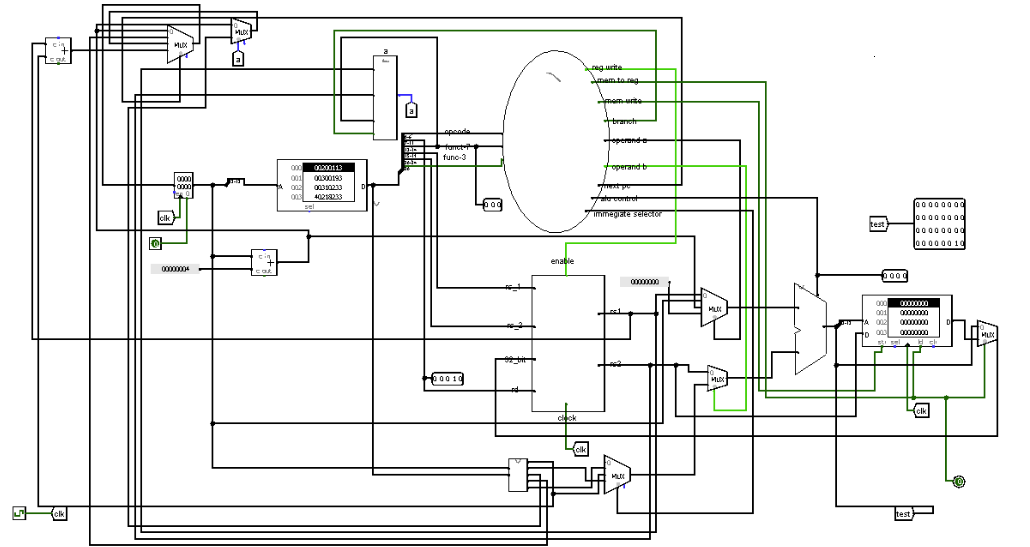
\includegraphics[scale=0.6]{RV32I Single Cycle.png}
    \caption{RV32I de Ciclo Único}
\end{figure}

\subsection{Adaptação da Unidade de Controle e Verificação do Funcionamento}

\newpage
\newpage

\begin{figure}[h]
    \centering
    \includegraphics[scale=0.6]{Pipelining de 5 estágios no LogSim.png}
    \caption{Pipelining de 5 estágios}
\end{figure}

A unidade de controle da CPU também passou por adaptações para coordenar adequadamente as operações vetoriais e garantir a sincronia entre os estágios do pipeline. A comunicação entre as unidades funcionais e os registradores vetoriais foi cuidadosamente gerenciada pela unidade de controle para garantir a correta execução das instruções vetoriais.

Após a implementação completa da extensão vetorial, a CPU foi submetida a testes e validações abrangentes. Foram criados testvectors para avaliar o funcionamento de todas as instruções escalares e vetoriais suportadas. Diversos cenários de execução foram simulados para verificar a estabilidade, precisão e eficiência da CPU em diferentes tipos de tarefas e cargas de trabalho.

\subsection{Códigos Verilog}

\subsubsection{32-bitAdder.v}
\begin{lstlisting}
module adder (clk,adr,a);


 reg [31:0]c=0;
 input [31:0]adr;
 output reg [31:0]a;
 input clk;

  
  
  always @(*) begin
     a = adr + 4;
  end
    
endmodule
\end{lstlisting}

\subsubsection{ALU}
\begin{lstlisting}
module ALU (
   op,op1,op2,res
); //Module ALU
   input [3:0]op;
   input [31:0]op1,op2;
   output reg signed [31:0]res ;


 always @* begin
      case (op)
         4'b0000 : res = op1 + op2; 
         4'b0001 : res = op1 - op2;
         4'b0010 : res = op1 & op2;
         4'b0011 : res = op1 | op2;
         4'b0100 : res = op1 ^ op2;
         4'b0101 : res = op1 << op2;
         4'b0110 : res = op1 >> op2;
         4'b0111 : res[0] = (op1 < op2) ? 1 : 0;
         4'b1000 : res[0] = ($signed (op1) < $signed (op2)) ? 1 : 0;
         4'b1001 : res = op1 >>> op2;
         4'b1111 : res = op1 ;
         default: res = 0;
      endcase
 end

endmodule
\end{lstlisting}


\subsubsection{Branch.v}
\begin{lstlisting}
module branch (
   op1,op2,fu_3,en,re
 );

 input [31:0]op1,op2;
 input [2:0]fu_3;
 input en;
 output reg re;
 wire fu_3;

 always @* begin
    if(en==1)begin
       case (fu_3)
          3'b000 : re = (op1 == op2) ? 1 : 0 ;
          3'b001 : re = (op1 != op2) ? 1 : 0 ;
          3'b100 : re = ($signed (op1) < $signed (op2)) ? 1 : 0 ;
          3'b101 : re = ($signed (op1) >= $signed (op2)) ? 1 : 0 ;
          3'b110 : re = (op1 < op2) ? 1 : 0 ;
          3'b111 : re = (op1 >= op2) ? 1 : 0 ;
       endcase
    end
 end
   
endmodule
\end{lstlisting}

\subsubsection{Byte.v}
\begin{lstlisting}
module byte_acces (
   byte_address,Byte_access,word
 );

 input [1:0]byte_address;
 input [31:0]word;
 output reg [7:0]Byte_access;

 always @(*) begin
   case (byte_address)
      2'b00 :  Byte_access = word[7:0];
      2'b01 :  Byte_access = word[15:8];
      2'b10 :  Byte_access = word[23:16];
      2'b11 :  Byte_access = word[31:24];
   endcase
 end
   
endmodule
\end{lstlisting}

\subsubsection{Immediate.v}
\begin{lstlisting}
module immediate (
   instruction,pc,I,S,SB,UJ,U
 );
 input signed [31:0]instruction,pc;
 output reg signed [31:0]S,SB,UJ,U,I,k,sb1 ;
 reg [11:0]II ,SS ,az;
 reg [20:0]ay;
 reg signed [31:0]ax ;

   always @(*) begin 
   az[0] = 1'b0;
   az[4:1] = instruction[11:8];
   az[10:5] = instruction[30:25];
   az[11] = instruction[7];
   az[12] = instruction[31];

   ay[0] = 1'b0;
   ay[10:1] = instruction[30:21];
   ay[11] = instruction[20];
   ay[19:12] = instruction[19:12];
   ay[20] = instruction[31];

   ax[19:0] = instruction[31:12];
   ax[31:20] = 0;

   II = instruction[31:20];
   I = {{20{II[11]}},II};
   SS[4:0] = instruction[11:7] ;
   SS[11:5] = instruction[31:25];
   S = {{20{SS[11]}},SS};
   sb1 = {{0{az[12]}},az};
   SB = pc + sb1;
   k = {{0{ay[21]}},ay};
   UJ = k + pc;
   U = ax << 12;
   end
endmodule
\end{lstlisting}

\subsubsection{TypeDecoder.v}
\begin{lstlisting}
module control (
   input [31:0]opcode,output reg [8:0]dec
 );
 reg [6:0]c ;
 reg [31:7]b;

 always @* begin
    c = opcode[6:0];
 end

 always @* begin
   case (c)
      7'b0110011 : dec = 9'b100000000;
      7'b0010011 : dec = 9'b010000000;
      7'b0000011 : dec = 9'b001000000;
      7'b0100011 : dec = 9'b000100000;
      7'b1100011 : dec = 9'b000010000;
      7'b1101111 : dec = 9'b000001000;
      7'b1100111 : dec = 9'b000000100;
      7'b0110111 : dec = 9'b000000010;
      7'b0010111 : dec = 9'b000000001; 
      default: dec = 0;
   endcase
end
endmodule
\end{lstlisting}

\subsubsection{controlunit.v}
\begin{lstlisting}
module unit (
   input [8:0]dec,input [31:0]in,output reg[14:0]un
 );

 reg [2:0]fun_3 ;
 reg fun_7;

 always @* begin
    fun_3 = in[14:12];
    fun_7 = in[30];
 end

 reg [3:0]a,c;
 reg [2:0]b,d;

 always @* begin
   a = dec[3:0];
   b = dec[4:2];
   c = dec[8:5];
   d[0] = dec[5];
   d[1] = dec[0] | dec[1];
   d[2] = dec[2] | dec[6] | dec[7];
 end
   
 always @* begin
   un[14] = dec[0] | dec[1] | dec[2] | dec[3] | dec[6] | dec[7] | dec[8];
   un[13] = dec[6];  //lw
   un[12] = dec[5];  //sw
   un[11] = dec[4];  //branch
   case (a)
      0001 : un[10:9] = 2'b01;
      0010 : un[10:9] = 2'b11;
      0100 : un[10:9] = 2'b10;
      1000 : un[10:9] = 2'b10;
      default: un[10:9] = 0;
   endcase
   un[8] = dec[0] | dec[1] | dec[5] | dec[7] | dec[6] | dec[2];
   case (b)
      3'b001 : un[7:6] = 2'b11;
      3'b010 : un[7:6] = 2'b01;
      3'b100 : un[7:6] = 2'b10; 
      default: un[7:6] = 0; 
   endcase
   if (dec == 9'b100000000) begin
      if (fun_7==1) begin
         case (fun_3)
            3'b000: un[5:2] = 4'b0001;
            3'b100: un[5:2] = 4'b0101;
            3'b010: un[5:2] = 4'b0111;
            3'b110: un[5:2] = 4'b0011;
            3'b001: un[5:2] = 4'b1101;
            3'b101: un[5:2] = 4'b1001; 
            3'b011: un[5:2] = 4'b1001;
            3'b111: un[5:2] = 4'b0011;
            default:un[5:2] = 0; 
         endcase

      end else begin                                //fun-7 = 0 
         case (fun_3)                          
            3'b000: un[5:2] = 4'b0000;
            3'b100: un[5:2] = 4'b0100;
            3'b010: un[5:2] = 4'b0111;
            3'b110: un[5:2] = 4'b0011;
            3'b001: un[5:2] = 4'b0101;
            3'b101: un[5:2] = 4'b0110; 
            3'b011: un[5:2] = 4'b1000;
            3'b111: un[5:2] = 4'b0010;
            default : un[5:2] = 0;
         endcase
      end
      
   end
   if (dec == 9'b010000000) begin
      if (fun_7==1) begin
         case (fun_3)
            3'b000: un[5:2] = 4'b0000;
            3'b100: un[5:2] = 4'b0100;
            3'b010: un[5:2] = 4'b0111;
            3'b110: un[5:2] = 4'b0011;
            3'b001: un[5:2] = 4'b1101;
            3'b101: un[5:2] = 4'b1001; 
            3'b011: un[5:2] = 4'b1000;
            3'b111: un[5:2] = 4'b0010;
            default:un[5:2] = 0; 
         endcase

      end else begin                                //fun-7 = 0 
         case (fun_3)                          
            3'b000: un[5:2] = 4'b0000;
            3'b100: un[5:2] = 4'b0100;
            3'b010: un[5:2] = 4'b0111;
            3'b110: un[5:2] = 4'b0011;
            3'b001: un[5:2] = 4'b0101;
            3'b101: un[5:2] = 4'b0110; 
            3'b011: un[5:2] = 4'b1000;
            3'b111: un[5:2] = 4'b0010;
            default:un[5:2] = 0;
         endcase
      end
   end
   if (dec == 9'b001000000 ) begin
      if (fun_3 == 3'b010) begin
         un[5:2] = 4'b0000;
      end
   end
   if (dec == 9'b000100000 & fun_3 == 3'b010) begin
      un[5:2] = 4'b0000;
   end
   if (dec == 9'b000001000 ) begin
      un[5:2] = 4'b1111;
   end
   if (dec == 9'b000000100 & fun_3 == 3'b000) begin
      un[5:2] = 4'b1111;
   end
   if (dec == 9'b000000010 ) begin
      un[5:2] = 4'b0000;
   end
   if (dec == 9'b000000001) begin
      un[5:2] = 4'b0000;
   end
   case (d)
      3'b001 : un[1:0] = 2'b11;
      3'b010 : un[1:0] = 2'b01;
      3'b100 : un[1:0] = 2'b10; 
      default: un[1:0] = 0;
   endcase
 end
endmodule
\end{lstlisting}

\subsubsection{datamemory.v}
\begin{lstlisting}
module data_mem (
    clk,addr,d,str,ld,resu
 );

 input clk,str,ld;
 input [31:0]addr,d;
 output logic [31:0] resu;
 reg [11:0]ad1 ;
 logic [31:0] data_rom[1024-1:0];
   
 always @(clk) begin
    if (str) begin
       data_rom[addr] <= d;
    end
    if (ld) begin
      resu = data_rom[addr];
   end
 end

endmodule
\end{lstlisting}

\subsubsection{instructionmemory.v}
\begin{lstlisting}
module ram #(
   parameter address = 12, size = 32
 ) (
    clk,addre,din,dout,we
 );
    input clk,we;
    input [31:0]din;
    input [11:0]addre;
    output reg [31:0]dout ;

    reg [31:0] mem[2**address-1:0] ;

    initial begin
        $readmemh("coef.mem",mem);
    end
    
    always @(*) begin
       if (we==1) begin
          mem[addre]=din;
       end 
       else begin
          dout = mem[addre];
       end
         
    end
endmodule
\end{lstlisting}

\subsubsection{mux1-2.v}
\begin{lstlisting}
module mux1_2 (
   sel,a,b,c
 );
   input sel;
   input [31:0]a,b;
   output reg [31:0]c ;

 always @* begin
   case (sel)
      1'b0 : c = a;
      1'b1 : c = b; 
      
   endcase
 end
endmodule
\end{lstlisting}

\subsubsection{mux2-4.v}
\begin{lstlisting}
module mux2_4 (
   sel,a,b,c,d,o
 );

 input [1:0]sel;
 input [31:0]a,b,c,d;
 output reg [31:0]o ;

 always @* begin
   case (sel)
      2'b00 : o = a;
      2'b01 : o = b;
      2'b10 : o = c;
      2'b11 : o = d; 
   endcase
 end
   
endmodule
\end{lstlisting}

\subsubsection{}



\section{Resultados}

\begin{figure}[h]
    \centering
    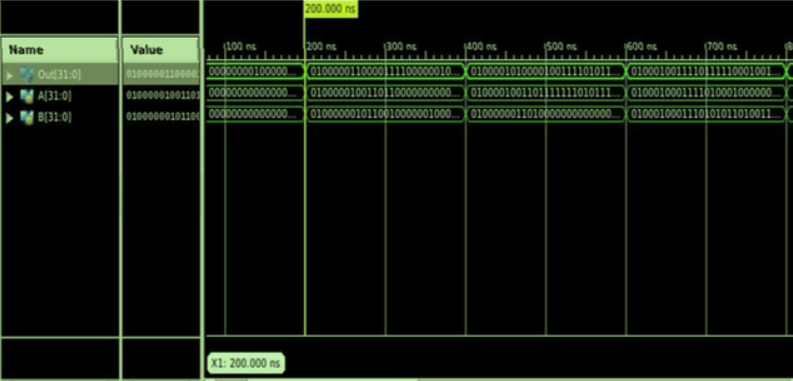
\includegraphics[scale=0.6]{Testbench simulação CPU 32 bits com instruções vetoriais.png}
    \caption{Testbench simulação CPU 32 bits com instruções vetoriais}
\end{figure}

A extensão da CPU RISC-V de 32 bits para suportar instruções vetoriais resultou em uma solução eficiente e poderosa para aplicações que demandam processamento intensivo de dados. As operações vetoriais permitiram um aumento significativo no desempenho, especialmente em tarefas que podem ser paralelizadas.

\subsection{Considerações Finais}


O desenvolvimento desta CPU RISC-V com suporte a instruções vetoriais representa um avanço significativo no campo da computação de alto desempenho. A utilização de instruções vetoriais abre novas possibilidades para a aceleração de algoritmos e aplicações complexas, permitindo que sejam realizadas operações em grandes conjuntos de dados de forma mais eficiente.

A implementação bem-sucedida da extensão vetorial nesta CPU ressalta a viabilidade e o potencial das arquiteturas RISC-V em lidar com tarefas de computação intensivas. O conhecimento adquirido neste projeto pode ser aplicado em futuras pesquisas e projetos no campo da arquitetura de computadores, possibilitando a contínua inovação e aprimoramento das CPUs RISC-V em aplicações do mundo real.

\section{Referências}

\begin{enumerate}
\item \textit{Computer Organization and Design RISC-V Edition: The Hardware Software Interface}, 2nd edition, by David A. Patterson and John L. Hennessy. Morgan Kaufmann, 2021.

\item \textit{Computer Organization and Architecture: Designing for Performance}, 11th edition, by William Stallings. Pearson, 2022.

\item \textit{Digital Design Using VHDL: A Systems Approach} by John F. Wakerly. Pearson, 2016.

\end{enumerate}

\end{document}